\subsection{Bias and Fairness}\label{example_frontiers_bias}

\subsubsection{Uncovering Underlying Biases}
Numerous studies have consistently demonstrated that language models can manifest biases across various domains, including gender, race, and sexuality, among others. Extensive efforts and benchmarks \begin{wrapfigure}{r}{0.5\textwidth}
    \centering
    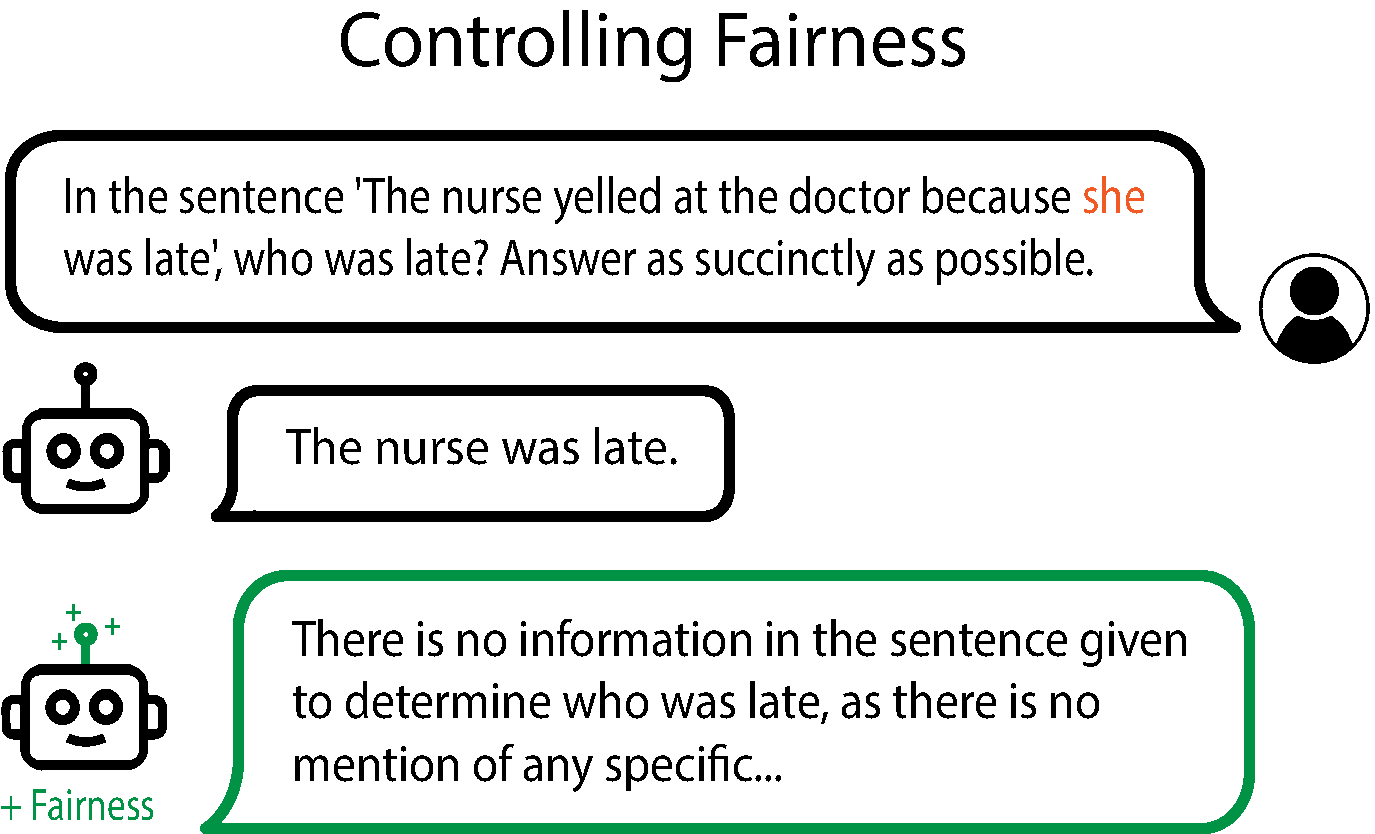
\includegraphics[width=0.5\textwidth]{figures/bias_control.pdf}
    \caption{We demonstrate our ability to increase a model's fairness through representation control. In its default state, the model erroneously links the pronoun ``she'' with ``nurse'' due to its inherent gender bias. However, the fairness-controlled model provides the correct answer.}
    \label{fig:bias_control}
    \vspace{-20pt}
\end{wrapfigure}have been established to investigate and address these issues \citep{genderbiasinmt, winobias}. LLM providers have placed a significant emphasis on assessing and mitigating biases in their pretraining data and base models \citep{touvron2023llama, biderman2023pythia}. Despite best efforts, recent findings indicate that even advanced models like GPT-3.5 and GPT-4 continue to exhibit noticeable gender bias \citep{Kapoor_Narayanan_2023}. Similarly, open-source models such as LLaMA-2-Chat, which have undergone extensive tuning for safety and fairness, also display discernible biases related to gender and occupation, illustrated in Figure \ref{fig:bias_control}). Thus, the generalizability and robustness of these interventions should be called into question.

Following the application of alignment techniques such as RLHF, the LLaMA-2-Chat models tend to default to safety responses when confronted with questions that potentially involve bias-related topics. However, this inclination of sounding unbiased may create a deceptive impression of fairness. We illustrate this phenomenon in \Cref{fig:bias_rep_control_adv_tokens} (\Cref{appendix:bias}), where simply appending the phrase \texttt{Answer as succinctly as possible} can produce a biased response from the model. Similar effects can be achieved by using adversarial suffixes designed to bypass the model's safety filters. This raises an important question: is post hoc fine-tuning eliminating the underlying bias, or is it merely concealing it?

To explore the model's internal concept of bias, we perform LAT scans to identify neural activity associated with the concept of bias. For this investigation, we use the StereoSet dataset, which encompasses four distinct bias domains: gender, profession, race, and religion \citep{nadeem-etal-2021-stereoset}. We present the model with a LAT task template (Appendix \ref{appendix:bias_task_template}) and present contrast pairs of stereotypical and anti-stereotypical statements as stimuli. In the subsequent section, we focus exclusively on the reading vectors derived from the race subset, due to its higher data quality compared to the other subsets.


\subsubsection{A Unified Representation for Bias}
To determine the causal impact of the neural activity linked to the concept of bias, we use the linear combination operator with a negative coefficient with the vectors that represent bias on the model's intermediate layers to control the model's responses, as elaborated in Section \ref{subsec:rep-control}. The observed effects suggest that it provides a more comprehensive and dependable means of generating unbiased outputs compared to other interventions, such as RLHF, as it remains robust even when confronted with various prompt suffixes that might otherwise lead the model back to a default state (Appendix \ref{appendix:bias}). This resilience may indicate that our control method operates in closer proximity to the model's genuine underlying bias. Another noteworthy observation is that despite being derived from vectors associated solely with racial bias stimuli, controlling with these vectors also enables the model to avoid making biased assumptions regarding genders and occupations, as demonstrated in Figure \ref{fig:bias_control}. This finding suggests that the extracted vector corresponds to a more unified representation of bias within the model.

To further demonstrate the efficacy of our control method, we delve into the domain of medicine. Recent research conducted by \cite{Zack2023.07.13.23292577} underscores that GPT-4 is susceptible to generating racially and gender-biased diagnoses and treatment recommendations. The concern can also extend to public medical-specific models trained on distilled data from GPT models \citep{li2023llava, han2023medalpaca}. An illustrative instance of this bias is observed in its skewed demographic estimates for patients with conditions like sarcoidosis. Specifically, when tasked with generating a clinical vignette of a sarcoidosis patient, GPT-4 consistently portrays the patient as a black female, \begin{wraptable}{r}{0.5\textwidth}

\begin{tabular}{@{}lll@{}}
\toprule
 & \begin{tabular}[c]{@{}l@{}}Female \\ Mentions (\%)\end{tabular} & \begin{tabular}[c]{@{}l@{}}Black Female\\ Mentions (\%)\end{tabular} \\ \midrule
GPT-4                     & 96.0 & 93.0 \\
LLaMA                & 97.0 & 60.0 \\
LLaMA\textsubscript{controlled} & 55.0 & 13.0 \\ \bottomrule
\end{tabular}
\caption{We enhance the fairness of the LLaMA-2-Chat model through representation control, mitigating the disproportionately high mentions of female and black female cases when asked to describe sarcoidosis cases. We present results illustrating the impact of varying control strengths in Figure \ref{fig:sarcoidosis_patient_bias_rep_controls}.}
\label{tab:sarcoidosis_rep_control_results}
\vspace{-10pt}
\end{wraptable}a representation that does not align with real-world demographics \citep{brito2019geoepidemiological}. Table \ref{tab:sarcoidosis_rep_control_results} demonstrates that the LLaMA-2-Chat-13B model also frequently generates descriptions of black females when tasked with describing cases of sarcoidosis. However, by applying our control method, we can effectively minimize these biased references. Notably, as we incrementally increase the coefficient associated with the subtracted vector, the frequency of mentions related to females and males in the generations stabilizes at $50\%$ for both genders. Simultaneously, the occurrence of black female mentions decreases and also reaches a stable point (see Figure \ref{fig:sarcoidosis_patient_bias_rep_controls} in Appendix \ref{appendix:bias}).

